

\subsection{Derivatives CR-14}

\subsubsection{Derivatives market}
\begin{itemize}
\item \textbf{Counterparty credit risk}
\begin{itemize}
    \item Derivatives transactions: represent contractual agreements either to make payments or to buy or sell an underlying security at a time or times in the future.
    \begin{itemize}
        \item Financial institutions, mainly banks, provide derivative contracts to their end user clients and hedge their risks with one another.
        \item are dominated by a relatively small number of large counterparties(dealers)许多市场都被数量相对较少的大型交易方所控制
    \end{itemize}
   \item Counterparty credit risk: the possibility that a counterparty may not meet its contractual requirements under the contract when they become due.
\end{itemize}


\item \textbf{OTC vs. Exchange}\\
\begin{tabular}{|p{5cm}|p{5cm}|p{5cm}|}
    \hline
    &\textbf{Exchange-traded} & \textbf{Over-the-counter (OTC)} \\
    \hline
    \textbf{Terms of contract} & Standardised (maturity, size, strike, etc.) & Flexible and negotiable \\
    \hline
    \textbf{Maturity} & Standard maturities, typically at most a few months & Negotiable and non-standard, often many years \\
    \hline
    \textbf{Liquidity} & Very good & Limited and sometimes very poor for non-standard or complex products \\
    \hline
\end{tabular}



\item \textbf{Clearing}
\begin{itemize}
    \item \textbf{Execution}: buyer and seller enter into a legal obligation to buy/sell securities or another underlying
    \item \textbf{Clearing}: Transaction is managed prior to settlement (margining, cashflow payments, etc.)
    \item \textbf{Settlement}: Transaction is settled via exchange of securities and/or cash and legal obligations are therefore fulfilled.
    \item Since it requires a certain amount of standardisation, not all OTC derivatives can be centrally cleared.
    \item The main OTC derivatives are: interest rate (and inflation) derivatives, foreign exchange derivatives, equity derivatives, commodity derivatives, and credit derivatives
\end{itemize}





\item \textbf{Participants}

\begin{itemize}
    \item \textbf{Large player}:large global bank, often known as a dealer.
    \begin{itemize}
        \item Have a vast number of derivatives trades on their books and have many clients and other counterparties
        \item Trade across all asset classes and will collateralize positions
        \item Will be a member of most or all exchanges and CCP to facilitate trading on their own account and for their clients.
    \end{itemize}
    \item \textbf{Medium-sized player}: a smaller bank or other financial institution
    \begin{itemize}
        \item Smaller number of clients and counterparties
        \item Will be a member of local exchanges and may be a member of a number of global ones
    \end{itemize}
    \item \textbf{End user}: a large corporate, sovereign, or smaller financial institution with derivatives requirements
    \begin{itemize}
        \item Overall position will be very directional
        \item Unwilling to commit to margining or posting collateral
    \end{itemize}
    \item \textbf{Third parties}: may offer settlement/margining/collateral management, software, trade compression, and clearing services.

\end{itemize}







\item \textbf{Collateral}
\begin{itemize}
    \item Exchange-traded derivatives: are effectively settled on a daily.
    \begin{itemize}
        \item most simple, liquid, and short-dated derivatives. Margin must be posted against losses on a daily basis
    \end{itemize}
    \item OTC derivatives: may be collateralized
    \begin{itemize}
        \item OTC centrally cleared: Daily collateralization in cash (variation margin)
        \item OTC collateralized: bilateral OTC derivatives. Parties post collateral(which may be cash or securities) to one another in order to mitigate the counterparty risk.
        \item OTC uncollateralized: parties do not post collateral (or post less and/or lower quality collateral)
    \end{itemize}
    \item Banks and end users
    \begin{itemize}
        \item 头寸具有方向性，盯市价值及现金流波动大The overall
        portfolio will typically be directional. The value of the derivatives, or mark-to-market(MTM)volatility will be significant and any associated margin or collateral flows may vary substantially.
        \item 一对一对冲敞口而非整体宏观对冲敞口 End users may
        hedge risks on a one-for-one basis rather than macro basis.
        \item The hedging needs may lead to certain imbalances
    \end{itemize}
\begin{figure}[H]
    \centering
    
\includegraphics[width=0.8\textwidth]{enduser.jpg}
\end{figure}



\end{itemize}


\item \textbf{ISDA}
\begin{itemize}
    \item The International Swaps and Derivatives Association (ISDA) is a trade organization for OTC derivatives practitioners.
    \begin{itemize}
        \item Standard legal documentation to increase efficiency and reduce aspects such as counterparty risk
        \item The ISDA Master Agreement主协议：the market standard for OTC derivative documentation
    \end{itemize}
    \item Master agreement
    \begin{itemize}
    \item Bilateral framework which contains terms and conditions
    \item Multiple transactions will be covered under a general Master Agreement to form a single legal contract of an indefinite term, covering many or all of the transactions.
    \item Core section核心部分+a schedule containing adjustable terms附表组(可调整条款)
    \item 合约条款涉及：netting, collateral, termination events, the definition of default, and the close-out process
    \end{itemize}
\item 交易对手风险视角，ISDA主协议具有以下降低风险的特
点：
\begin{itemize}
\item The contractual terms regarding the posting of collateral有
关抵押品的合同条款
\item Events of default and termination违约事件和终止
\item All transactions referenced are combined into a single net obligation所有参考交易合并为单一净债务
\item The mechanics around the close-out process are defined确定平仓机制
\end{itemize}
\item ISDA主协议涵盖的违约事件有：
\begin{itemize}
\item Failure to pay or deliver未付款或未交付
\item Breach of agreement违背合约
\item Credit support default(collateral terms)信用支持违约
\item Misrepresentation错误陈述
\item Default under the specified transaction特定交易下的违约
\item Cross-default(default on another obligation)交叉违约
\item Bankruptcy
\item Merger without assumption不承担义务的合并
\end{itemize}
\item May lead to the loss for the nondefaulting party:
\begin{itemize}
\item The total value of the transactions to the nondefaulting party is positive and greater than the collateral (if any) posted by the defaulting party.非违约方价值为正，但违约方缴纳的抵质押物不足
\item The total value of the transactions is positive to the defaulting party and the collateral posted by the nondefaulting party is greater than this value.违约方价值为正，未为违约方缴纳抵质押物超过合约价值
\end{itemize}
\end{itemize}
\end{itemize}

\subsubsection{CCP and modeling derivatives risk}


\begin{itemize}
    \item \textbf{Systemic risk}: A major concern with respect to OTC
    derivatives is systemic risk, which generally refers to an
    uncontained crisis which may cause the failure of an entire financial system or market.系统性风险一般是指可能导致整
    个金融系统或市场崩溃的无法控制的危机
    \item \textbf{Special purpose vehicle特殊目的实体}
    Special purpose vehicle (SPV) or special purpose entity (SPE) is a legal entity(e.g.a company or limited partnership) created typically to isolate a firm from financial risk.
    \begin{itemize}
        \item To isolate counterparty risk.
        \item SPVs aim essentially to change bankruptcy rules
        \begin{itemize}
            \item Shift priorities 改变清偿顺序
        \end{itemize}
        \item An SPV transforms counterparty risk into legal risk.
        \begin{itemize}
            \item A bankruptcy court to combine the SPV assets with those of the originator
        \end{itemize}   
    \end{itemize}
   \item \textbf{Derivatives product companies衍生品公司}
   \begin{itemize}
    \item DPCs are generally triple-A-rated entities set up by one or more banks as a bankruptcy-remote subsidiary of a major dealer由一家或多家银行设立的三A级实体，作为主要交易商的破产远程子公司
    \begin{itemize}
   \item Provides external counterparties with a degree of
   protection against counterparty risk by protecting against
   the failure of the DPC parent.通过防止DPC母公司倒闭
\end{itemize}

\item Maintained a triple-A rating
\begin{itemize}
    \item Minimizing market risk(Mirror trades: matched book)
    \item Support from a parent: If the parent were to default, then the DPC would either pass to another well-capitalized institution or be terminated
    \item Credit risk management and operational guidelines:
    Restrictions were also imposed on(external) counterparty
    credit quality and activities(position limits, margin, etc.)
\end{itemize}

\item However, was such a triple-A entity of a double-A or worse bank really a better counterparty than the bank itself?
\begin{itemize}
    \item The GFC essentially killed the already-declining world of DPCs.
    \item A DPC's fate inextricably with that of its parent. DPCs的命运与其母公司的命运密不可分地联系在一起
\end{itemize}

\end{itemize}

\item Monolines and CDPCs单一险种公司
\begin{itemize}
    \item Monoline insurance companies: were financial guarantee companies with strong credit ratings that were utilized to provide 'credit wraps', which are financial guarantees.
    \item Credit derivative product companies(CDPCs):were an extension of the DPC concept that had business models similar to those of monolines.
    \item When the GFC developed through 2007, monolines experienced major problems due to the MTM-based valuation losses on the insurance they had sold.
\end{itemize}

\item Central clearing of OTC derivatives
\begin{itemize}
\item From the late 1990s, several major CCPs began to provide
clearing and settlement services for OTC derivatives and other
non-exchange-traded products (repo).
\begin{itemize}
\item These OTC transactions are still negotiated privately and off-exchange, but are then novated into a CCP on a post-trade basis.这些场外交易仍然是私下和场外谈判的，但在交易后被更替到中央交易对等中心
\end{itemize}
\item In 2009, the G20 leaders agreed in Pittsburgh to require:
\begin{itemize}
\item All standardized OTC derivatives to be traded on exchanges or electronic platforms
\item Mandatory central clearing of standardized OTC derivatives
\item The reporting of OTC derivatives to trade repositories向交易资料库报告场外衍生工具
\item Higher capital requirements for non-centrally cleared OTC derivatives.提高非集中清算场外衍生品的资本要求
\end{itemize}
\item Central clearing of OTC derivatives- the roles
\begin{itemize}
\item To sets certain standards and rules for its clearing members
制定一定的标准和规则
\item To take responsibility for closing out all the positions of a defaulting clearing member负责平仓违约会员头寸
\item To maintain financial resources to cover losses in the event of a clearing member default:
\begin{itemize}
    \item Variation margin: closely track market movements
    \item Initial margin: cover the worst-case liquidation or close-out costs above the variation margin
    \item A default fund: mutualize losses in the event of a severe default
\end{itemize}
\item To have a documented plan for the very extreme situation
when all their financial resources (initial margin and the
default fund) are depleted全部耗尽
\begin{itemize}
    \item Additional calls to the default fund
    \item Variation margin haircutting
    \item Selective tear-up of positions
\end{itemize}
\item CCPs provide a number of benefits:Allow netting of all trades executed through CCPs
\begin{itemize}
    \item CCPs manage margin requirements from their members to reduce the risk associated with the movement in the value of their underlying portfolios.
    \item The CCP absorbs the 'domino effect’by acting as a sort of financial shock absorber充当金融冲击吸收器来吸收"多米诺骨牌效应“(Auctioning the defaulted members' positions)
\end{itemize}
\end{itemize}
\end{itemize}

\item Bilateral margin requirements
\begin{itemize}
    \item Whilst clearing is mandatory, it can be avoided by trading contracts that are not sufficiently standardized to be cleared
    \item Regulators introduced mandatory margin(collateral) rules for derivatives that would remain bilateral.双边合约也进入了强制保证金制度
\end{itemize}



\item Derivatives risk modelling
\begin{itemize}
    \item VaR
    \begin{itemize}
        \item VaR does not give an indication of the possible loss outside the confidence level chosen
        \item VaR is that it is not a coherent risk measure (not behave in a sub-additive fashion)
    \end{itemize}
    \item ES: not ignoring completely the impact of large losses; coherent risk measure
    \item Models: the financial markets have a somewhat love/hate relationship with mathematical models.
    \begin{itemize}
        \item The quantitative modelling of counterparty risk is complex and prone to misinterpretation and misuse.
        \item Counterparty risk involves looking years into the future rather than just a few days, which creates further complexity that is not to be underestimated.交易对手风险涉及未来数年而非短短几天
    \end{itemize}
    \item Correlation and dependency: counterparty risk takes
    difficulties with correlation to another level.
\end{itemize}



\end{itemize}


\subsection{Counterparty Risk CR-15}


\subsubsection{Definition of counterparty risk}
\begin{itemize}
 \item Counterparty credit risk is the risk that the entity with whom one has entered into a financial contract (the counterparty) will fail to fulfil their side of the contractual agreement.
 \begin{itemize}
    \item Over-the-counter (OTC) derivatives
    \item Bilaterally cleared
    \item Uncollateralized
 \end{itemize}
\end{itemize}

\subsubsection{Lending risk vs. counterparty risk}
\begin{itemize}
\item Lending risk:
\begin{itemize}
    \item Notional amount at risk during lending period is usually known with a degree of certainty.
    \item Only one party takes lending risk. (i.e. bondholder).
\end{itemize}
 \item Counterparty risk:
\begin{itemize}
    \item The value of the contract in the future is uncertain.
    \item Since the value of the contract can be positive or negative, counterparty risk is typically bilateral.
\end{itemize}
\end{itemize}


\subsubsection{Settlement, pre-settlement, and margin period of risk}
\begin{itemize}
    \item Pre-settlement risk: a counterparty will default prior to the final settlement of the transaction. (counterparty risk)
    \begin{itemize}
    \item Long-dated OTC derivatives
    \end{itemize}
     \item Settlement risk: arises at settlement times due to timing differences between when each party performs its obligations under the contract.
    \begin{itemize}
    \item Occurs for only a small amount of time(days or even hours)
    \item A very large exposure(potentially 100of the notional)
    \item Spot contracts现货合同；FX markets外汇市场
    \end{itemize}

    \item Margin period of risk(MPoR): the risk horizon when
    collateralized/margined

    \begin{itemize}
    \item Collateralized bilateral OTC derivatives: 10 business days
    \item Centrally-cleared OTC derivatives: 5 business days
    \end{itemize}



\end{itemize}

\subsubsection{Institutions and transactions}
\begin{itemize}
    \item Large global banks have exposure to all asset classes
    \item Smaller banks may have more limited exposure
    \item End users may also have limited exposure
    \item Counterparty risk faced with CCPs may receive attention over the coming years
\end{itemize}



\subsubsection{Mitigations of counterparty risk}
\begin{itemize}
    \item Netting: Bilateral netting agreements allow cashflows to be offset and,in the event of default
    \item Collateral: Collateral agreements specify the contractual posting of cash or securities against MTM losses.
    \item Hedging: hedging counterparty risk with instruments such as credit default swaps(CDSs).
    \item Central counterparties: CCP act as intermediaries to centralize counterparty risk between market participants.
    \item Other contractual clauses: resets or additional termination.
\end{itemize}


\subsection{Netting, Close-out and Related Aspects CR-16}

\subsubsection{Cash flow netting}
\begin{itemize}
    \item International Swaps and Derivatives Association (ISDA)
    \begin{itemize}
    \item The market standard for OTC derivative documentation is the ISDA Master Agreement, which was first introduced in 1985 and is now used by the majority of market participants to document their OTC derivative transactions.
    \begin{itemize}
    \item Aims to remove legal uncertainties and to provide mechanisms for mitigating counterparty risk.
    \end{itemize}
    \end{itemize}
\item Payment netting:involves the netting of different payments between two counterparties that are(generally denominated in the same currency).
\begin{itemize}
    \item Reduces the time and costs associated with making payments
    \item Reduce operational risk, counterparty and liquidity risk
\end{itemize}
\item Currency netting and CLS
\begin{itemize}
\item Settlement risk is also a major consideration in foreign
exchange(FX) markets, where the settlement of a contract
involves payment of one currency against receiving the other.
(Herstatt risk赫斯塔特风险)
\item Non-deliverable forward (NDF) transaction: currency exchange is cash-settled based on the difference between the NDF rate and the prevailing spot FX rate applied to the notional.
\end{itemize}
\item Continuous linked settlement(CLS): reduce settlement risk in FX transactions across a range of eligible currencies
\begin{itemize}
    \item Payment versus payment(PVP):Only after both currencies have arrived does CLS Bank make the outgoing payment to A and B.
\end{itemize}
\item Clearing rings: multilateral netting before the development of central clearing.
\begin{itemize}
    \item Three or more members who would agree to "ring out" offsetting positions.
    \item Participants in the ring had to be willing to accept substitutes for their original counterparties.
\end{itemize}

\begin{center}
    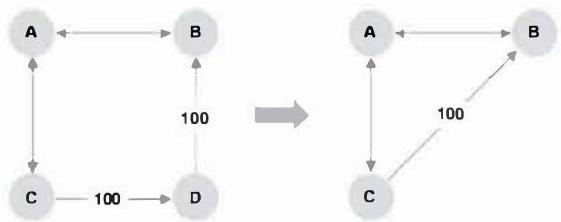
\includegraphics[width=0.4\textwidth]{images/0196660e-d86d-7ef6-8951-a48e2a482302_18_549_222_561_222_0.jpg}
    \end{center}
    \hspace*{3em} 
\item Multilateral netting
\begin{itemize}
\item Portfolio compression: achieves multilateral netting benefits via the cooperation of multiple counterparties that partially or entirely eliminate transactions.
\begin{itemize}
    \item Aims to minimize gross notional of positions in the market
\end{itemize}

\item Portfolio compression:
\begin{itemize}
    \item Preserve the market risk position of participants
    \item Reducing non-market risks such as settlement and counterparty risk.
    \item Reduce operational costs and may also lower systemic risk
\end{itemize}
\begin{center}
    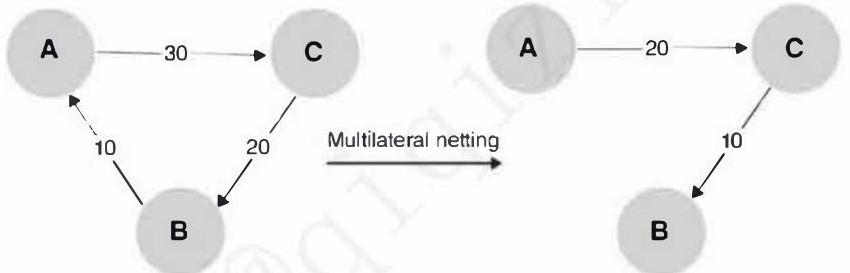
\includegraphics[width=0.7\textwidth]{images/0196660e-d86d-7ef6-8951-a48e2a482302_18_399_1033_850_273_0.jpg}
    \end{center}
    \hspace*{3em} 

\item Compression cycle works: an algorithm is run to determine changes to transactions that generate multilateral netting benefits, but keeping each participant's portfolio neutral in terms of value and risk.用算法来对交易的修改，产生多边
净额结算利益，保持每个参与者在价值和风险方面的中性
\begin{itemize}
    \item Participants can specify constraints (internal credit limits of a participant).
    \item Basic portfolio compression by its nature requires standard contracts
\end{itemize}
\item Compression Algorithm
\begin{itemize}
    \item It is not clear what should be minimized.
    \item An obvious choice may be the total notional.
    \item Alternative choices could be to use the squared notional or the total number of positions, which would reduce large exposure and interconnectedness respectively.
\end{itemize}

\end{itemize}

\item Benefits of cash flow netting
\begin{itemize}
    \item Operational costs: By reducing the number of cash flows and transactions, operational costs can be reduced.
    \item Legal risks: Portfolio compression may reduce legal risk by contractually simplifying portfolios and not relying on future risk mitigation.
    \item Regulatory: some simple regulatory methodologies are partially based on gross notional and will, therefore, appear more benefcial if these values are reduced
\end{itemize}



\end{itemize}


\subsubsection{Value netting}

\begin{itemize}
\item Close-out netting终止净额结算/净额交割
\begin{itemize}
    \item Close-out netting: comes into force in the event that a counterparty defaults, and aims to allow a timely termination and settlement of the net value of all transactions with that counterparty.及时终止和结算与违约方的所有交易的净值
    \begin{itemize}
    \item Close-out: the right to terminate transactions with the defaulted counterparty and cease any contractual payments
    \item Netting: the right to offset the value across transactions and determine a net balance for the final close-out amount.
    \end{itemize}
\item For the surviving party:
\begin{itemize}
    \item Owes money: makes this payment
    \item Is owed money: makes a bankruptcy claim for that amount.
\end{itemize}

\item Jump to the bankruptcy queue for all but its net exposure
\item It only depends on mark-to-market(MTM) values at the time of default and not matching cashflows

\item Close-out netting and ISDA
\begin{itemize}
    \item Payment netting reduces settlement risk, close-out netting is relevant to counterparty risk since it reduces pre-settlement risk.
    \item Close-out netting reduces the complexity involved in the close-out of transactions in the event that a counterparty defaults.
    \item The ISDA has obtained legal opinions supporting the close-out and netting provisions in their Master Agreements in most relevant jurisdictions.
    \item Determining a close-out amount:
    \begin{itemize}
    \item Firm or indicative quotations for replacement transactions supplied by one or more third parties由一个或多个第三方提供的替换交易的确定或指示性报价
    \item Relevant market data supplied by one or more third parties
    \item From internal sources
    \end{itemize}
\end{itemize}

\item Set-off冲销
\begin{itemize}
    \item Netting across product categories(e.g. OTC derivatives and loans) is not definitely possible as they are documented differently.
    \item 银行既给交易对手提供利率互换服务，同时又提供浮动利率贷款，但内部两个交易是分开的，在违约的情况下两者价值是否可以抵消

\item Set-off vs. netting:经济效果上相同，但含义不同
\begin{itemize}
    \item Set-off: recognizes the existence of cross-claims
    \item Netting: results in a single contractual claim
\end{itemize}
\end{itemize}

\end{itemize}


\item The impact of netting
\begin{itemize}
    \item 风险降低Risk reduction:
    \begin{itemize}
    \item Close-out netting is risk mitigant for counterparty risk
    \item Has been critical for the growth of the OTC derivatives market.
    \end{itemize}
\item 波动大，可能有系统崩溃风险Netted positions are
inherently more volatile than their underlying gross positions,which can create systemic risk
\item 改变市场参与者对特定交易对手风险增加的看法If credit
exposures were driven by gross positions, then all those
trading with the troubled counterparty would have strong
incentives to attempt to terminate existing positions and stop
any new trading.
\item Netting impact on other creditors
\begin{itemize}
    \item Netting redistributes value to OTC derivatives creditors from other creditors
    \item Netting redistributes value to OTC derivatives creditors from other creditors.
\end{itemize}
\item Multilateral netting and Bifurcation
\begin{itemize}
\item Bifurcation分歧：between cleared and bilateral transactions
\begin{itemize} 
\item Market participants executing offsetting transactions since one product may be clearable and the other not.
\item An increase in overall exposure caused by multilateral netting related to central clearing of only a subset of trades
\end{itemize}
\end{itemize}



\end{itemize}




\item Additional termination event (ATE)

\begin{itemize}
    \item Additional termination event(ATE): is designed to mitigate against counterparty risk by allowing a party to terminate transactions or apply other risk reducing actions when their counterparty's credit quality is deteriorating.
    \item 触发事件
    \begin{itemize}
    \item Rating downgrade (e.g. below investment grade)
    \item For unrated parties such as hedge funds: market capitalisation, net asset value, or key person departure may be used.
    \end{itemize}
    \item 触发后果不一定是直接终止合约
    \begin{itemize}
    \item Provide a replacement counterparty
    \item Provide a counterparty offering a third-party guarantee
    \item Terminate the transaction(s) at their current replacement value 按目前的重置价值终止交易
    \item Post some sort of margin
    \end{itemize}
\item Potential danger of ATE
\begin{itemize}
    \item Risk-reducing benefit: a systematic deterioration in credit quality is much harder to nullify.系统性恶化很难消除
    \item Weaknesses in credit ratings评级反应迟钝
    \item Cliff-edge effects: single-notch rating downgrade may cause a dramatic consequence.下调一个等级，可能会造
    成巨大的后果
    \item Modelling difficulty: rating transitions probability cannot be implied from market data
\end{itemize}


\end{itemize}


\end{itemize}





\subsection{Margin (Collateral) and Settlement CR-17}
\subsubsection{Margin terms}
\begin{itemize}
    \item Rationale for collateral 
    \begin{itemize}
    \item Counterparties
    \begin{itemize}
    \item In the case of a positive value:a party will call for margin
    \item In the case of negative value: a party will be required to post margin themselves
    \end{itemize}
\item Terminology
\begin{itemize}
    \item Collateral: used for OTC derivatives markets and contractual agreements such as ISDA Master Agreement场外市场用更多
    \item Margin:used for exchange-traded markets to represent a similar concept 场内市场用更多
\end{itemize}
\item The fundamental idea of OTC derivatives collateralization is that cash or securities are passed (with or without actual ownership changing) from one party to another primarily as a means to reduce counterparty risk.
\begin{itemize}
    \item 场外市场的抵质押物可以是现金、证券甚至是非金融资产
    \item Counterparty risk, in theory, can be completely neutralized as long as a sufficient amount of margin is held against it.
\end{itemize}



\end{itemize}

\item Margins
\begin{itemize}
    \item Variation margin: members who have lost money pay their loss amount to the exchange CCP, while members who have gained receive their gain amount from the exchange CCP.(Reflects current exposure)
    \begin{itemize}
        \item MPoR(margin period of risk): effective delay in receiving margin
        \begin{itemize}
        \item The inherent delay in the process between the time the party last posted margin and the time they were declared in default最后一次交保证金到违约间的延迟
        \item The associated costs in replacing and/or rehedging defaulted transactions.替换和/或重新安排违约交易的 相关费用
        \end{itemize}
    \end{itemize}
\item Initial margin: funds or marketable securities that must be deposited with the CCP in addition to variation margin.
\begin{itemize}
    \item Extra margin that must be posted independently from the value of the underlying portfolio.
    \item For OTC derivatives, use the term 'Independent amount'.
    \item Reflects potential future exposure
    \begin{itemize}
    \item 99 confidence interval over a 10-day horizon(incorporates a period of significant financial stress).
    \end{itemize}
\end{itemize}
\end{itemize}
\item OTC derivatives market
\begin{itemize}
    \item Bilateral OTC derivatives market: has used margin almost entirely in the form of variation margin, and initial margin(independent amount) has been quite rare.场外市场，交换变动保证金，比较少交初始保证金
\begin{itemize}
    \item Initial margin is a much more common concept on
    derivative exchanges and central counterparties (CCPs).
\end{itemize}
    \item Regulation covering margin-posting in bilateral markets is making initial margin more common.
    \item Uncleared margin requirements (UMR): regulators have
    started to impose bilateral margin requirements
    \begin{itemize}
    \item Reduction of systemic risk: reducing “contagion and spillover effects”减少传染和溢出效应
    \item Promotion of central clearing:aligning costs(notably initial margin)双边清算成本和中央清算成本一直，促进中央清算的采用
    \end{itemize}
    \item Apply to all OTC derivatives(FX swaps and forwards)
\end{itemize}


\item Credit support annex(CSA)
\begin{itemize}
    \item Within an ISDA Master Agreement, it is possible to append a Credit Support Annex(CSA) where the parties agree to contractual margin-posting.
    \item No CSA:最典型的是银行和end user(corporate)
    \item Two-way CSA:For two financial counterparties, a two-way CSA is more typical, where both parties agree to post margin.
    \item One-way CSA: only one party can receive collateral
    \begin{itemize}
    \item A high-quality entity such as a triple-a sovereign or supranational trading with a bank.
    \item Additional risk for the collateral giver
    \end{itemize}



\end{itemize}


\item Margin term
\begin{itemize}
    \item Threshold: is the amount below which margin(collateral) is not required, leading to undercollateralization.
    \begin{itemize}
    \item If the MTM is above the threshold, only the incremental amount of collateral can be called for.
    \item Threshold=0: collateral would be posted under any circumstance
    \item Threshold <0: post initial margin
    \item Threshold ∞:counterparty will not post collateral under any circumstance.
    \end{itemize}
    \item Minimum transfer amount (MTA): is the smallest amount of margin that can be transferred.
    \begin{itemize}
    \item Represents a balance between risk mitigation versus operational workload.平衡风险缓释与业务工作量
      \end{itemize}
    \item Rounding 取整：A collateral call or return amount may also be rounded to a multiple of a certain size to avoid dealing with awkward quantities.
  
 \item Types of collateral
 \begin{itemize}
  \item Partially collateralized: reduction of exposure is imperfect.(Threshold can be seen as approximately capping the exposure.)
  \item Strongly collateralized: assume thresholds are zero and therefore the exposure is reduced significantly.
  \item Overcollateralized:assume initial margin and therefore the exposure is reduced further.
 \end{itemize}



\end{itemize}
\item Credit support amount
\begin{itemize}
\item Within the CSA, two parties can choose a number of key
parameters and terms that will define the margin-posting
requirements in detal.
 \item Credit support amount: the amount of margin that may be requested at a given point in time.
 \begin{itemize}
 \item Variation margin is captured and the initial margin is referred to separately as independent amount.上述金额表达的是变动保证金，初始保证金并不囊括在内
 \end{itemize}
\end{itemize}

\item Margin types and haircuts
\begin{itemize}
\item Haircuts 折减率：acts as a discount to the value of the margin and provides a cushion in the event that the security is sold at a lower price.
\item Extra margin must be posted which acts as an overcollateralization to mitigate against a drop in the value of the asset
\item Cash: no haircuts
\item Defined as fixed percentage amounts
\end{itemize}

\end{itemize}







\subsubsection{Impact of margin}

\begin{itemize}
    \item Valuation agent估值代理
    \begin{itemize}
    \item Valuation agent: the party calling for the delivery or return of margin and must handle all calculations.
    \item The role of valuation agent:
    \begin{itemize}
    \item Calculate the current value, market value of margin (adjusted by haircuts), uncollateralized exposure and credit support amount
    \end{itemize}
\item dispute over a margin call is common.
\begin{itemize}
\item Margin disputes are not relevant for centrally-cleared
transactions since CCP is the valuation agent.
\item Reconciliations: aim to minimize the change of a dispute
by agreeing on valuations and margin requirements across
portfolio.

\begin{itemize}
    \item Various third parties also offer services around valuation,exchange of margin, dispute management, and portfolio reconciliation.
\end{itemize}


\end{itemize}

\end{itemize}

\item Impact of margin on exposure
\begin{itemize}
\item Why margin cannot perfectly mitigate exposure
\begin{itemize}
\item The presence of a threshold means that a certain amount of exposure cannot be collateralized.阈值导致无法足值抵押
\item The delay in receiving margin and parameters such as the minimum transfer amount create a discrete effect 由于 MTA保证金并非连续的，而是离散的
\item Initial margin can be thought of as making the threshold negative and can potentially reduce the exposure to zero.
\end{itemize}
\item Impact on other creditors: margin does not reduce risk, it merely redistributes it. Other creditors will be more exposed




\end{itemize}



\item Rehypothecation and Segregation
\begin{itemize}
    \item Rehypothecation再抵押：the reuse of securities or cash margin by the margin receiver(e.g.in another margin
    agreement or a repo transaction).
    \begin{itemize}
    \item For variation margin: rehypothecation is important in OTC derivatives markets where many parties have multiple hedges and offsetting transactions
    \end{itemize}

\item Segregation分离：aims to ensure that margin posted is legally protected in the event that the receiving party becomes insolvent.
\begin{itemize}
\item For initial margin: segregation can avoid there being additional counterparty risk in relation to the initial margin posted.
\item Whilst safer from the point of view of counterparty risk, segregation does create higher funding costs.
\end{itemize}

\item Segregated margin can be held:
\begin{itemize}
\item Held directly by the margin receiver
\item Held by a third party acting on behalf of one party
\item Held in tri-party custody where a third party holds the margin
\end{itemize}




\end{itemize}  


\item Potential problems of margin
\begin{itemize}
    \item Liquidity risk: in the event that margin has to be liquidated following the default of a counterparty, the non-defaulting party faces transaction costs and market volatility over the liquidation period.在交易对手违约后必须清算保证金的情况下，非违约方在清算期间将面临交易成本和市场波动。
    \item FX risk: margin posted in cash or securities denominated in a currency that does not match the currency or currencies of the portfolio保证金与有关投资组合计价货币不一致
    \item Legal risk: rehypothecation and segregation are subject to possible legal risks
    \item Operational risk: can be especially significant for the largest banks, which may have thousands of relatively nonstandardized margin agreements with clients, requiring
    posting and receipt of billions of dollars of margin on a given day.它们可能与客户签订了数千份相对非标准化的保证金协议，需要在特定的一天缴纳和收取数十亿美元的保证金。
    \item Funding liquidity risk:increasing collateralization may reduce counterparty risk, but it increases funding liquidity risk.
    \begin{itemize}
        \item Potential risk arising from the difficulty to raise required funding in the future, especially when margin needs to be segregated and/or cannot be rehypothecated.
    \end{itemize}


\end{itemize}

\end{itemize}




\subsection{Central Clearing CR-18}
\subsubsection{volution and mechanics}

\begin{itemize}
    \item Evolution of complete clearing
    \begin{itemize}
    \item Direct clearing   
    \item Clearing rings: three or more counterparties could“ring out” offsetting positions
    \item Complete clearing: a central counterparty (CCP) is placed centrally between all counterparties and assumes all such contractual rights and responsibilities
    \end{itemize}

\item What is a CCP?
\begin{itemize}
    \item CCP:is a particular financial market infrastructure (FMI) that represents a set of rules and operational arrangements designed to allocate, manage, and reduce counterparty risk in a bilateral market.是一种特殊的金融市场基础设施(FMI),代表了一套旨在分配、管理和降低双边市场中交易对手风
    险的规则和操作安排。
\begin{itemize}
    \item Can reduce the interconnectedness within financial
    markets相互关联性
    \item Can provide more transparency on the positions
\end{itemize}
\item The true CCP landscape is much more complex than
represented
\begin{itemize}
\item Client clearing:不能成为CCP会员的交易对手需要通过CCP会员清算
\item Bilateral trades:不是所有衍生品都适合
\item Multiple CCPs:全球有许多不同的CCP
\begin{itemize}
\item Regional:为本地清算以本币计价的交易；监管
\item Product:专注某些产品类型
\end{itemize}

\end{itemize}

  \item Clearing relationships
  \begin{itemize}
  \item CCP members: large global banks and some other very
  large financial institutions
  \begin{itemize}
      \item Smaller banks, buy-side and other financial firms, and other non-financial end users are unlikely to be direct clearing
  \end{itemize}
  \item Requirement: admission criteria; financial commitment;
  operational
\end{itemize}

\end{itemize}

\item Novation
\begin{itemize}
    \item Novation: means that the CCP essentially steps in between parties to a transaction and therefore acts as an insurer of counterparty risk in both directions.
    \begin{itemize}
        \item Buyer to the seller and seller to the buyer
        \item Matched book:
        \begin{itemize}
            \item No net market risk
            \item Take the counterparty risk
        \end{itemize}
    \end{itemize}
  \item Portfolio compression vs. CCP
  \begin{itemize}
      \item  Portfolio compression: requires actual transactions(or cash flows) to be eliminated
      \item CCP can compress risk, whereas bilateral compression can only compress objective quantities such as cash flows.
  \end{itemize}

\end{itemize}

\end{itemize}



\subsubsection{CCP risk management}

\begin{itemize}
    \item Functions of CCP
    \begin{itemize}
        \item Multilateral offset: provide netting and/or compression benefits
        \item Loss absorbency损失吸收能力
        \item Default management: hedging, auctioning, allocating loss, transferring client trades
    \end{itemize}
\item CCP membership requirements
\begin{itemize}
    \item Creditworthiness: the probability of default of the clearing member, as assessed by external or internal methods.
    \item Liquidity: the ability of the member to meet liquidity requirements, such as the need to meet margin calls at short notice.可以短时间内满足追加保证金要求
    \item Operationality: the ability to adhere to the CCP rules, such as those pertaining to auctions.
\end{itemize}
\item Margin and default funds
\begin{itemize}
    \item Variation margin: be transferred on a daily (and sometimes intradaily) and must usually be in cash
    \begin{itemize}
    \item Requires timely and reliable price data for all cleared derivatives and, where price data is not directly available, market-standard valuation methods.可靠的价格数据或市场标准的估值方法
    \end{itemize}
\item Initial margin: requirements may also frequently change with market conditions and must be provided in cash or liquid
    assets (e.g. treasury bonds).
    \begin{itemize}
    \item Cover potential close-out losses in the event of a default by that clearing member.
    \item Is calculated using different scenarios for possible price movements over an assumed close-out period (MPoR or liquidation period), such as five days.
    \end{itemize}

\item Default funds: CCP members all contribute to a CCP
    \begin{itemize}
    \item Loss mutualization: losses above the resources contributed by the defaulter are shared between CCP members.
    \end{itemize}
 
    \begin{table}[h]
        \centering
        \begin{tabular}{|p{5cm}|p{5cm}|p{5cm}|}
            \hline
            & \textbf{Higher initial margin} & \textbf{Lower initial margin} \\
            \hline
            \textbf{Cost} & Higher & Lower \\
            \hline
            \textbf{Client clearing} & Clients pay for their own risk via initial margin, promotes portability & Clients do not pay for their own risk directly, portability difficult \\
            \hline
            \textbf{Moral hazard} & Lower & Higher \\
            \hline
        \end{tabular}
        \caption{Comparison of Initial Margin and Default Fund}
    \end{table}
\item CPs are typically required to calibrate the size of the total default fund qualitatively via pre-defined stress tests. CCP通常需要通过预先确定的压力测试，定性地校准总违约基金的规模
\begin{itemize}
    \item Allocated to clearing members
\end{itemize}

\end{itemize}



\item Default scenarios and margin period of risk
\begin{itemize}
    \item  In a default scenario, the CCP neutralizes its exposure through:
    \begin{itemize}
        \item Macro-hedging宏观对冲
        \item Auctions 拍卖
        \begin{itemize}
        \item Sub-portfolio拆分成子组合拍卖
        \item Surviving CCP members bid the best price未违约会员还是有很强动力参与拍卖，把不利后果压倒最低
        \end{itemize}
        \item Fire drills:消防演习，定期进行违约管理程序演习，最大程度提高潜在拍卖效率
        \item Driving test:驾驶考试，对新成员进行测试
    \end{itemize}
\end{itemize}

\item The Loss Waterfall
\begin{itemize}
    \item Skin-in-the-game: equity contribution from the CCP
    \begin{figure}[h]
        \centering
        
\includegraphics[width=0.4\textwidth]{waterfall.jpg}
        \caption{Loss Waterfall}
    \end{figure}

\item Losses wiping out a significant portion of the default fund
\begin{itemize}
    \item Rights of assessment评估权：an unfunded obligation to contribute additionally to a default fund that has been depleted by losses
    \item Variation margin gains haircutting(VMGH)变动保证金扣减
    \item Tear-up强行终止合约，打破原有的matched book
    \item Forced allocation把反向交易强行给到未违约会员
    \end{itemize}
\end{itemize}


\item Impact of central clearing 
\begin{itemize}
    \item Advantages

\begin{itemize}
    \item Transparency
    \item Multilateral offset
    \item Loss mutualization
    \item Legal and operational efficiency
    \item Liquidity
    \item Default management
\end{itemize}
\item Disadvantages
\begin{itemize}
    \item Moral hazard
    \item Adverse selection
    \item Bifurcations清算标准产品的要求可能会在清算交易和非清算交易之间造成分歧
    \item Procyclicality 市场波动或危机的时候提高保证金要求
\end{itemize}


\end{itemize}


\end{itemize}



\subsection{Future Value and Exposure CR-19}
\subsubsection{Metrics for Credlit Exnosure}
\begin{itemize}
    \item Credit Exposure
    \begin{itemize}
        \item Definition: effective value of the relevant contracts at the default
        \item Credit Exposure = max(value,0)
        \begin{itemize}
        \item Loans:the credit exposure is the notional amount and is fixed.
        \item Swap, option and forward: the credit exposure is the value of the asset if it is positive.
        \item Futures and short options: the credit exposure is zero
        \end{itemize}
\item Characteristics affects credit exposure:
    \begin{itemize}
        \item Volatility
        \item Time horizon
        \item Risk mitigants
    \end{itemize}

    \begin{center}
        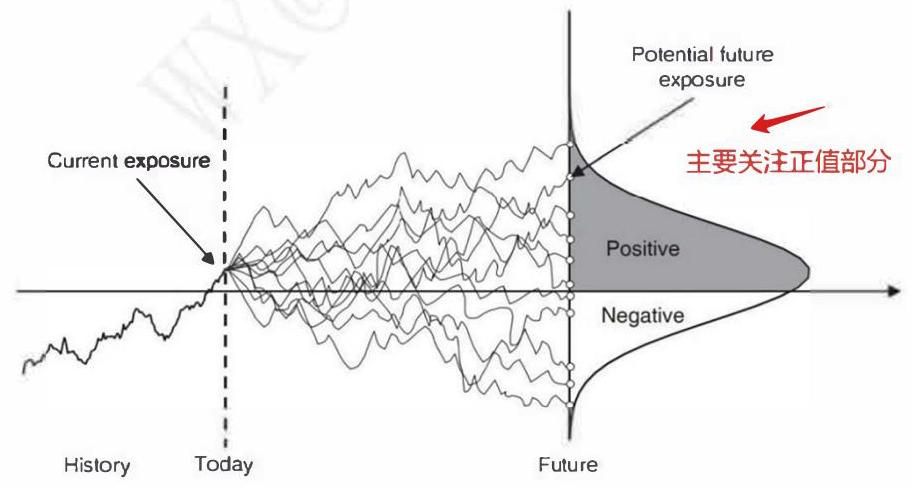
\includegraphics[width=0.7\textwidth]{images/0196660e-d86d-7ef6-8951-a48e2a482302_31_362_1335_911_487_0.jpg}
        \end{center}
        \hspace*{3em} 

    \end{itemize}
    
    \item Nature of exposure
    \begin{itemize}
        \item Asymmetric risk profile
        \begin{itemize}
        \item Exposure is similar to an option payoff, a key aspect will be volatility (of the value of the relevant contracts and margin)
        \item Options are relatively complex to price敞口量化也有其复杂性
        \end{itemize}
\item VaR vs.quantifying exposure
\begin{itemize}
    \item Time horizon: VaR-short horizon
    \begin{itemize}
    \item The “ageing” of transaction (cash flows, termination events, exercise decisions, and margin postings)
    \item When looking at longer time horizons, the trend (also known as the 'drift') of market variables is relevant
    \end{itemize}
    \item Risk mitigants考虑净额结算和保证金的影响
    \item Application:exposure must be defind for both risk management and pricing(i.e.xVA)传统方法偏向风控
\end{itemize}
    \end{itemize}
    

\item Metrics for Exposure
\begin{itemize}
\item Expected future value(EFV):对敞口分布求期望
\begin{itemize}
    \item Represents the expected (average) of the future value calculated with some probability distribution.
    \item At time zero: the current value
    \item EFV may vary significantly from current value
    \begin{itemize}
        \item Cash flow differential 比如利率互换交叉货币互换
        \item Forward rates: can differ significantly from current spot variables
        \item Asymmetric margin agreements: one-way CSA
    \end{itemize}
\end{itemize}
\end{itemize}


\item Potential future exposure(PFE):at a confidence level of x\%未来某个时期出现较坏的风险敞口是多少
\begin{itemize}
    \item Is an equivalent metric to VaR
    \item The highest (or lowest) exposure calculated to some underlying confidence level
\end{itemize}

\item Expected positive exposure(EPE): the average of all of the positive exposure.正敞口的平均数(负的取零)
\begin{itemize}
    \item Also referred to as “expected exposure(EE)”
\end{itemize}
\item Expected negative exposure(ENE): the average of all of the negative exposures.负敞口的平均数(正的取零)
\begin{itemize}
    \item Represents the positive exposure from the counterparty's point of view.
    \item Also referred to as “negative expected exposure(NEE)”
\end{itemize}
\item Average EPE:the average exposure across all time horizons.
\begin{itemize}
    \item The weighted average of the EPE across time.
    \item Also called a “loan equivalent”: the average amount effectively lent to the counterparty
\end{itemize}

\end{itemize}






\subsubsection{Exposure profile of various securities}

\begin{itemize}
\item Loans and Bonds

    \begin{itemize}
        \item 敞口几乎是确定的， 敞口大致等于名义价值
    \end{itemize}

\item forward contract 远期合约
\begin{itemize}
    \item The exposure is a rather simple increasing function reflecting the fact that， as time passes， there is increasing uncertainty about the value of the final exchange. 【随着时间推移，最终合约价值的不确定性不断增加】
\end{itemize}


\begin{center}
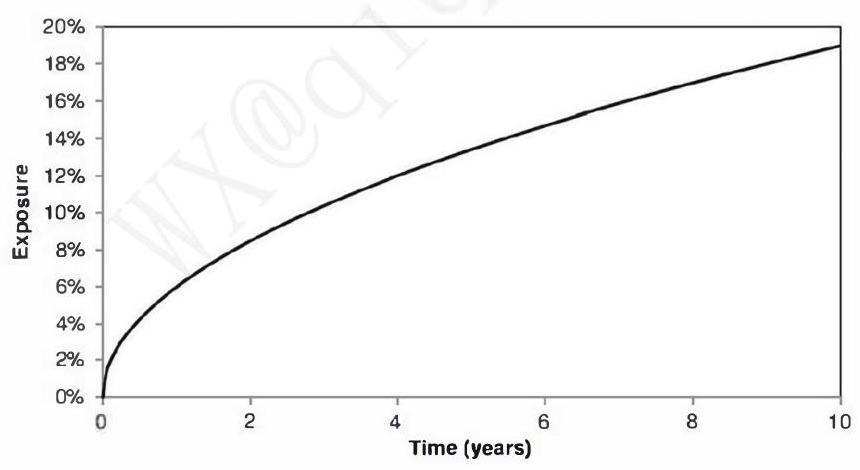
\includegraphics[width=0.7\textwidth]{images/0196660e-d86d-7ef6-8951-a48e2a482302_33_393_1199_860_470_0.jpg}
\end{center}
\hspace*{3em} 

\item Interest Rate Swap 利率互换
\begin{itemize}
    \item 浮动利率与固定利率的交换。期间换利息，期末换利息不换本金

    \item Exposure profile is characterized by a peaked shape.

    \item This peaked shape results from the balancing of future uncertainties over payments and the roll-off risk of swap payments over time.

\begin{center}
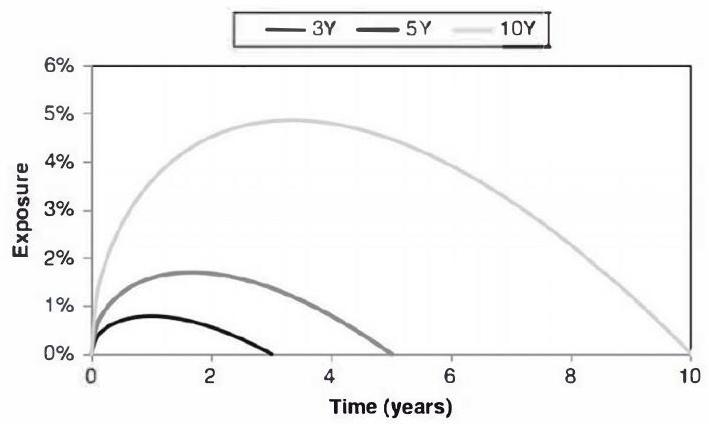
\includegraphics[width=0.6\textwidth]{images/0196660e-d86d-7ef6-8951-a48e2a482302_34_495_207_709_424_0.jpg}
\end{center}
\hspace*{3em} 

    \item 另外，有一些非标准化的利率互换可能不是同一个期限进行交割的，比如浮动利率(每三个月交换一次)交换固定利率(每六个月交换一次)， 此时现金流是不匹配的。【与普通利率互换敞口形状差不多，只不过是有点锯齿状】

\begin{center}
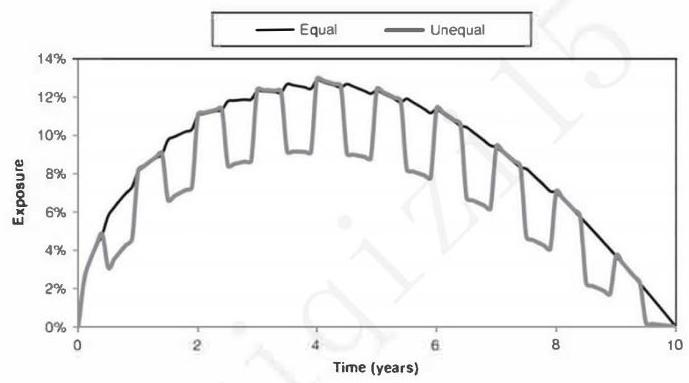
\includegraphics[width=0.5\textwidth]{images/0196660e-d86d-7ef6-8951-a48e2a482302_34_501_860_689_383_0.jpg}
\end{center}
\hspace*{3em} 

\item cross-currency swap 交叉货币互换
\begin{itemize}
    \item 就是一级学习的货币互换。

    \item 与利率互换不同，货币互换期间换利息，期末换利息和本金

    \item Some exposures come from interest rate risk (IR) while the majority results from the uncertainty with the final notional payment of FX rate risk.

    \item 也可以把货币互换看成是利率互换和外汇远期的结合。
\end{itemize}
\begin{center}
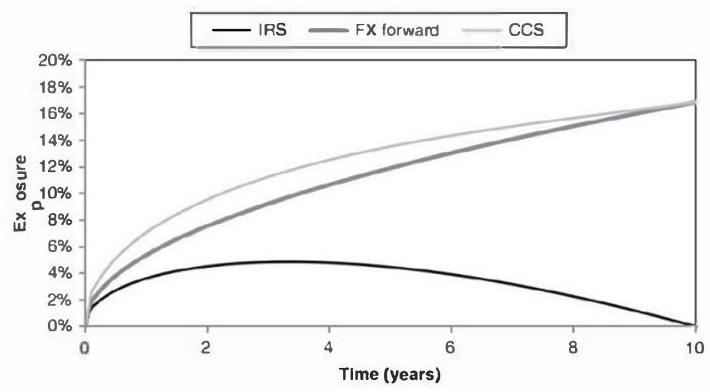
\includegraphics[width=0.6\textwidth]{images/0196660e-d86d-7ef6-8951-a48e2a482302_34_462_1661_710_392_0.jpg}
\end{center}
\hspace*{3em} 

\item CDS exposure:
\begin{itemize}
    \item EPE: shows a typical swap-like profile.

    \item  PFE: has a jump due to the default of the reference entity.
\end{itemize}
\begin{center}
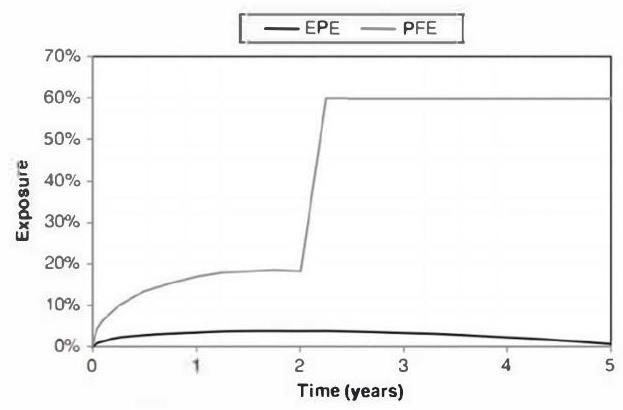
\includegraphics[width=0.5\textwidth]{images/0196660e-d86d-7ef6-8951-a48e2a482302_35_501_325_623_410_0.jpg}
\end{center}
\hspace*{3em} 

\item Swaption 和 forward starting swap
\begin{itemize}
    \item 补充知识:Swaption 和 forward starting swap 这两个产品，咱们没太关注过。 原版书在这里也并没有进行介绍， 直接介绍敞口。这里做一个知识补充:
    \begin{itemize}
        \item Swaption: 赋予持有人在未来某个日期或某段时间，进入一个 swap。是权利， 没有义务。
        \item Forward Starting Swap 是一种互换， 约定在未来某一日期开始生效。从那个日期起， 两方将在未来的若干时间段内交换一系列现金流。是权利也是义务， 必须要履行合约。
    \end{itemize}
    \item Swaption 会根据市场情况选择是否执行， forward starting swap 则是在未来某一特定日期开始执行。
    \item 在行权日期之前， swaption 的敞口总是大于 forward starting swap。
\end{itemize}
\item 在行权日期之后， 情况会反转， 因为在某些情况下， forward starting swap 可能有正值， 而 swaption 可能没有被行权(敞口下降)。
\end{itemize}

\begin{center}
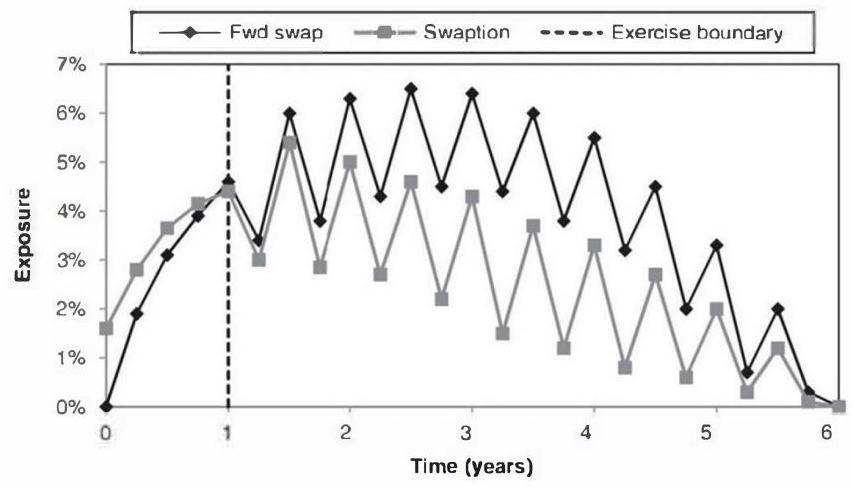
\includegraphics[width=0.7\textwidth]{images/0196660e-d86d-7ef6-8951-a48e2a482302_35_393_1493_852_487_0.jpg}
\end{center}
\hspace*{3em} 


\end{itemize}

\subsubsection{The impacts on exposure}
\begin{itemize}
    \item Reducing effect:the exposure profiles are partly offsetting(one is positive whilst the other is negative)
    \item Exposure
    \begin{itemize}
        \item Positive exposure:max(value -margin,0)
        \item Negative exposure:min(value -margin,0)
    \end{itemize}
   \item Collateralization is not a perfect form of risk mitigation
    \begin{itemize}
        \item Granularity effect: margin parameters such as thresholds and minimum transfer amounts
        \item Delay in receiving margin:MPoR
        \item Potential variation in the value of the margin itself
    \end{itemize}
    \item Funding, rehypothecation, and segregation
    \begin{itemize}
        \item Funding benefits and costs:Funding = value- margin
        \begin{itemize}
        \item Funding cost: term is positive
        \item Funding benefit:term is negative
        \item Posted margin: create a positive funding cost.
        \item Received margin: represent a benefit
        \end{itemize}
\item Various types of margin under certain situations\\

\begin{tabular}{|p{6cm}|p{3cm}|p{3cm}|}
    \hline
    & \textbf{降低交易对手风险} & \textbf{提供funding benefit} \\
    \hline
    Cash that does not need to be segregated & $\surd$ & $\surd$ \\
    \hline
    Securities that can be rehypothecated & $\surd$ (前提是haircut足够) & $\surd$ \\
    \hline
    Cash or securities that must be segregated or cannot be rehypothecated & $\surd$ & $\times$ \\
    \hline
    Counterparty posting own bonds (that can be rehypothecated) & ? & $\surd$ \\
    \hline
\end{tabular}

\item Impact of margin on exposure and funding
\begin{itemize}
    \item Positive exposure = max(Value -VM-$IM^R$,0)
    \item Funding = value -VM+$IM^P$
    \item 信用敞口：收到保证金降低敞口，缴纳保证金增加敞口
    \item Funding:
    \begin{itemize}
        \item 初始保证金：segregation,无法提供funding benefit
        \item 变动保证金：假设可以使用，可提供funding benefit
    \end{itemize}
\end{itemize}



    \end{itemize}
    
\end{itemize}


\subsection{CVA CR-20}
\subsubsection{Credit Valuation Adjustment and xVA}
\begin{itemize}
    \item Cedit valuation adjustment (CVA): was originally introduced as an adjustment to the risk-free value of a derivative to account for potential default.
    \begin{itemize}
    \item A dealer calculates CVA for each counterparty with which it has bilaterally cleared OTC derivatives.
    \item CVA is one’s expected loss from a default by the counterparty.在无风险价值上做调整(Risky value = Risk-free value-CVA)
    \end{itemize}
\item Motivation and challenge of pricing counterparty risk
\begin{itemize}
    \item Motivation: CVA has become a key topic for banks due to the volatility of credit spreads, the associated accounting and capital requirements(Basel III).
    \item Challenge:cash flow not fully at risk due to partial offset with opposing cash flows
\end{itemize}

\item Credit limit vs. CVA
\begin{itemize}
    \item Credit limit: are a traditional tool to control
    the amount of risk to a given counterparty over time.
\begin{itemize}
    \item Counterparty risk can be diversified by limiting exposure to any given counterparty, sector, or region.
    \item Characterize the potential future exposure(PFE) over time and compare this with a pre-determined limit.
    \item Effectively favoring short-term exposures
    \item A transaction with low(high) profitability may be accepted (rejected) because the existing credit limit is small(large).
\end{itemize}

    \item CVA: By pricing counterparty risk through CVA, the question becomes whether it is profitable once the counterparty risk component has been “priced in”.
    \begin{itemize}
        \item CVA directly incorporates the credit risk of the
    counterparty and so defines a minimum revenue that
    should be achieved.
    \end{itemize}
    
    \item Three levels to assessing the counterparty risk of a
    transaction

    \begin{table}[h]
        \centering
        \begin{tabular}{|p{4cm}|p{6cm}|p{4cm}|}
            \hline
            \textbf{Level} & \textbf{Description} & \textbf{Examples} \\
            \hline
            Trade level & Incorporating all characteristics of the trade and associated risk factors such as the precise cash flows & e.g. maturity, currency, CVA \\
            \hline
            Counterparty level & Incorporating the impact of risk mitigants such as netting and margining & e.g. netting, collateral, CVA \\
            \hline
            Portfolio level & Consideration of the risk to all counterparties, knowing that only a small fraction may default in a given time period & e.g. large exposure and correlation, Credit limits \\
            \hline
        \end{tabular}
        \caption{Risk Levels and Descriptions}
    \end{table}


\item CVA:encourages minimizing the number of trading
counterparties since this maximizes the benefits of netting
\item Credit limits: encourage maximizing the number of trading to
encourage smaller exposures and diversification
\item CVA and credit limits are typically used together as
complementary ways to quantify and manage counterparty
risk.
\end{itemize}

\item xVA
\begin{itemize}
    \item Economic costs of a derivative
    \begin{itemize}
        \item Funding
        \item Collateral
        \item Initial margin
        \item Regulatory capital
    \end{itemize}
\item Components of xVA Terms

\begin{table}[h]
    \centering
    \begin{tabular}{|p{4cm}|p{4cm}|p{4cm}|}
        \hline
        \textbf{Risk Type} & \textbf{Market Component} & \textbf{Cost Component} \\
        \hline
        Counterparty risk & CVA/DVA & Credit exposure, Default probability \\
        \hline
        Funding & FVA, MVA & Valuation, Initial margin amount \\
        \hline
        Collateral & CoVA & Collateral amount, Collateral cost \\
        \hline
        Capital & KVA & Capital amount, Capital cost \\
        \hline
    \end{tabular}
    \caption{Risk Components and Their Terms}
\end{table}

\item Valuation adjustments

\begin{figure}[H]
    \centering
    
\includegraphics[width=0.8\textwidth]{XVA.jpg}
    \caption{Valuation Adjustments}
\end{figure}

\item replacement cost and credit exposure
\item Default probability, credit migration, and credit spreads
\item Recovery and loss given default
\item Funding, collateral, and capital costs
\end{itemize}


\end{itemize}



\subsubsection{CVA and DVA}

\begin{itemize}
    \item Unilateral CVA(UCVA)
\[
UCVA \approx -LGD \times \sum_{i=1}^{m} d(t_i) \times EPE(t_i) \times PD(t_{i-1}, t_i)
\]

\begin{itemize}
    \item \(d(t_i)\): 折现因子
    \item \(PD(t_{i-1}, t_i)\): 边际违约概率
    \item 假定没有wrong-way risk
\end{itemize}

\item CVA as a spread: adjust a rate paid or received as a running spread (per annum charge)
\[ UCVA \approx -average EPE \times spread \]
\begin{itemize}
    \item Credit component:the credit spread of the counterparty
    \item Market component:the exposure, or average EPE
\end{itemize}

\item Bilateral CVA(BCVA)
\begin{itemize}
    \item Debt valuation adjustment(DVA): is the mirror image of CVA(own credit risk).
    \begin{itemize}
        \item DVA is the expected cost to the counterparty
        \item DVA will oppose the CVA as a benefit.
       \item DVA term corresponds to fact that in cases where party themselves default, they will make a“gain” if a negative exposure.
       \item DVA creates “price symmetry”. Parties can agree on prices.
    \end{itemize}
    \item 交易对手A和交易对手B (My CVA is your DVA)

\begin{itemize}
    \item \( V_A = -V_B \)
    \item \( V_A + CVA_A + DVA_A \) (party A point of view)
    \item \( V_B + CVA_B + DVA_B \) (party B point of view)
    \item \( BCVA = CVA + DVA \)
    \item \( CVA_A = -DVA_B \)
    \item \( CVA_B = -DVA_A \)
    \item CVA 是一个负数
    \item DVA 是一个正数
\end{itemize}

\item CVA 和 DVA 计算

\[
CVA = -LGD_C \times \sum_{i=1}^{m} d(t_i) \times EPE(t_i) \times PD_C(t_{i-1}, t_i) \times [1 - PD_P(0, t_{i-1})]
\]

\[
DVA = -LGD_P \times \sum_{i=1}^{m} d(t_i) \times ENE(t_i) \times PD_P(t_{i-1}, t_i) \times [1 - PD_C(0, t_{i-1})]
\]

\begin{itemize}
    \item \( P \) is the party making the calculation
    \item \( C \) is its counterparty
    \item 注意加入考虑生存概率（有关协方差PE与原版生存概率处理的不同说明）
\end{itemize}

\item As spread
\[
BCVA \approx -average EPE \times Spread_c- average ENE \times Spread_p
\]
\begin{itemize}
    \item Assuming that average EPE=-average ENE
    \[BCVA \approx -EPE \times (Spread_c-Spread_p)\]
    \item Weaker counterparties would pay stronger counterparties in order to trade with them based on the differential in credit quality.
\end{itemize}


\end{itemize}


\end{itemize}




\subsubsection{CVA allocation}
\begin{itemize}
    \item Netting CVA
\begin{itemize}
    \item \textbf{Netting CVA:} Risk mitigants such as netting reduce the value of CVA.
    \item Under one netting agreement (netting set):
    \[
    CVA_{NS} \leq \sum_{i=1}^{n} CVA_i
    \]
    \item where \( CVA_{NS} \) is the total CVA of all transactions under the netting agreement and \( CVA_i \) is the stand-alone CVA for transaction \( i \).
    \item The above effect can be significant.
\end{itemize}

\item Incremental CVA

\begin{itemize}
    \item \textbf{Incremental CVA:} The CVA of a transaction \( i \) is calculated based on the incremental effect this transaction has on the netting set.
    \[
    CVA^{NS \to NS^*} = CVA^{NS^*} - CVA^{NS}
    \]
    \[
    = -LGD \times \sum_{i=1}^{m} EPE^{NS \to NS^*}(t, t_i) \times PD(t_{i-1}, t_i)
    \]
    \item Incremental EPE can be negative, due to beneficial netting effects.
    \item The incremental CVA is never higher than the standalone CVA without netting.
    \item The benefit of netting seen in incremental CVA of a new transaction also depends on the relative size of the new transaction.净额结算的好处还和交易本身规模有关
    \begin{itemize}
        \item As the transaction size increases, the netting benefit is lost, and CVA(or DVA) will approach the standalone value.
    \end{itemize}
    
\end{itemize}

\item Marginal CVA: break down a CVA for any number of netted
transactions into transaction-level contributions that sum to
total CVA.

\item Impacts on CVA
\begin{itemize}
    \item Spread curve: if upwards-sloping, flat and inverted credit curves all have the same cumulative PD at the five-year point, the marginal default probabilities differ substantially.
    \begin{itemize}
        \item Upwards sloping: largest CVA
        \item Inverted sloping: smallest CVA
    \end{itemize}
\item Credit spread: CVA increases with increasing credit spread.(In default, CVA may be zero.)
 \item Impact of recovery rate:increase the recovery rate will
reduce the value of CVA.
\item  Initial margin and threshold: a high coverage of initial margin is held, CVA can be assumed to be zero.
\item Variation margin:
\begin{itemize}
    \item MPoR/Cure period: It is typically 10 or 20 days.
\end{itemize}

\end{itemize}


\end{itemize}








\subsubsection{Wrong-way risk}
\begin{itemize}
    \item 定义
    \begin{itemize}
        \item Wrong-way risk (WWR):indicate an unfavorable dependence between exposure and counterparty credit quality.
        \begin{itemize}
            \item The exposure is high when counterparty is more likely to default and vice versa.
        \end{itemize}
        
        \item Right-way risk(RWR): cases where the dependence between exposure and credit quality is a favourable one.
        \begin{itemize}
            \item Right-way situations will reduce counterparty risk.
        \end{itemize}
    \end{itemize}
    \item Examples of WWR and RWR
    \begin{itemize}
        \item 看跌期权
        \begin{itemize}
            \item A公司向B公司购入以B公司的股票为标的的看跌期权，当B公司违约概率上升时，股票价格会下跌，此时A所购入的看跌期权的盈利上升，信用风险口上升。所以此时对于A来说是错路风险
        \end{itemize}

        \item 商品互换
        \begin{itemize}
            \item 以A公司与B公司的原油互换为例，A公司支付固定的原油价格，收到B公司所支付的浮动的原油价格，此时A公司是WWR还是RWR要根据B公司的具体情况进行判断。
            \item 如果B公司是原油的经销商，此时当原油价格上升，有利于B公司的经营发展，所以B公司的PD下降，并且A公司的获利也更大，信用口上升，所以此时A公司面临RWR。
            \item 如果B公司是航空公司，当原油价格上升时，B公司的经营成本上升，不利于B公司的经营发展，所以B公司的PD会上升，此时A公司的信用口也上升，面临WWR
        \end{itemize}


        \item 信用违约互换
        \begin{itemize}
            \item 公司向B公司购入信用违约互换。此信用违约互换的标
            的资产和B公司的信用质量高度正相关，当B公司信用质量恶化，B公司的违约概率上升，并且标的资产的信用质量也恶化，此时会产生两种情况：
            \begin{itemize}
                \item 当标的资产信用质量恶化，但没有发生违约时，CDS的保费会上升，A公司之前购入的CDS相对于当前市场价格是较低的，A公司是相对盈利的，信用敞口上升，A公司面临WWR。
                \item 当标的资产信用质量恶化且发生违约，则会触发信用违约互换的赔付机制，A公司的信用风险口也上升，面临WWR。
            \end{itemize}
        \end{itemize}

        \item 外汇产品
        \begin{itemize}
            \item A公司与美国政府进行货币互换的交易，A公司支付美元，收英镑，美国政府支付英镑，收美元。当美国市场出现萧条情况时，美元贬值，此时美国政府较易违约，并且美元贬值对于A公司来说是支出少，收入多，所以A公司的信用敞口上升，面临WWR
        \end{itemize}
        \item 利率产品
        \begin{itemize}
            \item 假设A银行进入支付浮动利息，收入固定利息的利率互换，B公司支付固定利息，收入浮动利息，当经济恶化时，市场利率下降，B公司的违约概率上升，并且A银行支付的浮动利息相对减少，A银行在此笔互换中盈利上升，信用敞口上升，面临WWR。
        \end{itemize}
    \end{itemize}



    \item WWR modelling
    \begin{itemize}
        \item Hazard rate (intensity) approaches: introduce a stochastic process for the credit spread. Conditional EPE will be calculated. (easy to use)
        \begin{itemize}
            \item Correlation: directly via historical time series of credit spreads and other relevant market variables.
            \item Weak dependence between exposure and default
        \end{itemize}
        \item Structural approaches: mapping the default distribution and exposure distribution onto a bivariate distribution.
        \begin{itemize}
            \item WWR: Positive dependency will lead to an early default time being coupled with a higher exposure
        \end{itemize}
        \item Parametric approaches: linking the default probability parametrically to the exposure using a simple, functional relationship.
        \begin{itemize}
            \item If the portfolio has historically shown high values together with larger than average credit spreads, then this will indicate WWR
        \end{itemize}
        \item Jump approaches: jump at default.
        \begin{itemize}
            \item E.g.:counterparty defaults with FX rate
            \item Implied jump is larger for better-rated sovereigns
            \item A default of a large corporation should be expected to have quite a significant impact on the local currency
        \end{itemize}
    \end{itemize}
    \item Collateralization and WWR
    \begin{itemize}
        \item WWR may also be present in terms of the relationship between the value of margin and the underlying exposure.可以定义为敞口和抵质押物价值的关系
        \begin{itemize}
            \item 敞口上升，抵质押物价值反倒下降
        \end{itemize}
        \item 例子：
        \begin{itemize}
            \item Payer interest rate swap collateralized with a high-quality government bond.（WWR:利率上升，敞口上升，抵质押物价格下降）
            \item Cross-currency swap collateralized by cash in one of the two underlying currencies. Margin is held in the currency being paid.(如：付美元利息，收日元利息，抵质押物为美元)（WWR:美元贬值，敞口上升，抵质押物价值下降）
        \end{itemize}



    \end{itemize}


    \item CCP and WWR
    \begin{itemize}
        \item CCPs tend to disassociate credit quality and exposure. CCPs are in danger of implicitly ignoring WWR.
        \item WWR increases with increasing credit quality
        \begin{itemize}
            \item A large dealer represents more WWR than a smaller and/or weaker credit quality counterparty.
            \item CCPs should require greater initial margin and default fund contributions from better-credit-quality and more-systemically-important members.信用质量较好的成员违约的可能性较小，但如果违约，影响可能会更严重。
        \end{itemize}
        \item CCPs face WWR on the margin they receive.
        \begin{itemize}
            \item Under pressure to accept a wide range of eligible securities for initial margin purposes.
            \item Adverse selection: clearing members(and clients) will naturally choose to post margin that has the greatest risk (relative to its haircut) and may also present the greatest WWR to a CCP
        \end{itemize}
    \end{itemize}


\end{itemize}










\subsection{Counterparty Credit Risk压力测试 CR-21}






\begin{itemize}
    \item 把 CCR 看成是 credit risk 和 market risk 的结合
    \end{itemize}
    
    \begin{itemize}
    \item CCR 的压力测试主要包括 EL 和 CVA 两个方面。
    \end{itemize}
    
    (1)贷款组合的压力测试
    
    \begin{itemize}
    \item stress test could take EAD and LGD as deterministic and focus on stresses where the PD is subject to a stress.
    \end{itemize}
    
    \begin{itemize}
    \item 压力情况下的 PD， 违约概率可以表示为汇率或者失业率等变量在压力情况下的函数
    \end{itemize}
    
    \[
    {\mathrm{{EL}}}_{\mathrm{s}} = \mathop{\sum }\limits_{{\mathrm{i} = 1}}^{\mathrm{N}}{\mathrm{{PD}}}_{\mathrm{i}}^{\mathrm{s}} \times  {\mathrm{{EAD}}}_{\mathrm{i}} \times  {\mathrm{{LGD}}}_{\mathrm{i}}
    \]
    
    \({\mathrm{{EL}}}_{\mathrm{s}}\) : Stressed EL
    
    \begin{itemize}
    \item 压力损失 Stress loss 表示为压力下的 EL 和无压力下的 EL 的差额:
    \end{itemize}
    
    Stress loss \(= {\mathrm{{EL}}}_{\mathrm{s}} - \mathrm{{EL}}\)
    
    (2)衍生产品组合的压力测试
    
    \begin{itemize}
    \item Average EPE multiplied by an alpha factor: allows CCR exposures to be placed in a portfolio credit model at a high percentile loss of the portfolio of exposures。【需要考虑压力下的 PD 和 EPE】
    \end{itemize}
    
    \[
    \mathrm{{EL}} = \mathop{\sum }\limits_{{\mathrm{i} = 1}}^{\mathrm{N}}{\mathrm{{PD}}}_{\mathrm{i}} \times  \alpha  \times  {\mathrm{{EPE}}}_{\mathrm{i}} \times  {\mathrm{{LGD}}}_{\mathrm{i}}
    \]
    
    \[
    {\mathrm{{EL}}}_{\mathrm{s}} = \mathop{\sum }\limits_{{\mathrm{i} = 1}}^{\mathrm{N}}{\mathrm{{PD}}}_{\mathrm{i}}^{\mathrm{s}} \times  \alpha  \times  {\mathrm{{EPE}}}_{\mathrm{i}}^{\mathrm{s}} \times  {\mathrm{{LGD}}}_{\mathrm{i}}
    \]
    
    \[
    \text{ Stress loss } = {\mathrm{{EL}}}_{\mathrm{s}} - \mathrm{{EL}}
    \]
    
    (3)CVA 的压力测试
    
    \[
    {\mathrm{{CVA}}}_{\mathrm{n}} = \mathop{\sum }\limits_{{\mathrm{n} = 1}}^{\mathrm{N}}{\mathrm{{LGD}}}_{\mathrm{n}} \times  \mathop{\sum }\limits_{{\mathrm{i} = 1}}^{\mathrm{m}}{\mathrm{{EE}}}_{\mathrm{n}}\left( {\mathrm{t}}_{\mathrm{i}}\right)  \times  {\mathrm{{PD}}}_{\mathrm{n}}\left( {{\mathrm{t}}_{\mathrm{i} - 1},{\mathrm{t}}_{\mathrm{i}}}\right)
    \]
    
    \[
    {\mathrm{{CVA}}}^{\mathrm{s}} = \mathop{\sum }\limits_{{\mathrm{n} = 1}}^{\mathrm{N}}{\mathrm{{LGD}}}_{\mathrm{n}} \times  \mathop{\sum }\limits_{{\mathrm{i} = 1}}^{\mathrm{m}}{\mathrm{{EPE}}}_{\mathrm{n}}^{\mathrm{s}}\left( {\mathrm{t}}_{\mathrm{i}}\right)  \times  {\mathrm{{PD}}}_{\mathrm{n}}^{\mathrm{s}}\left( {{\mathrm{t}}_{\mathrm{i} - 1},{\mathrm{t}}_{\mathrm{i}}}\right)
    \]
    
    \[
    \text{ Stress loss } = {\mathrm{{CVA}}}^{\mathrm{s}} - \mathrm{{CVA}}\text{ 。 }
    \]
    
    (4) Pitfalls in stress testing CCR
    
    \begin{itemize}
    \item 现在的压力测试， 仅限于当前敞口的压力测试
    \end{itemize}
    
    \begin{itemize}
    \item CCR 很少与贷款组合或交易头寸的压力测试结果在一个一致的框架中。
    \end{itemize}
    
    \begin{itemize}
    \item 对于 CCR 来说，使用 delta 敏感度来计算敞口变化是有问题的，因为 CCR 具有高度非线性特性。
    \end{itemize}